%Notes:Talk about what exactly a proxy server is
\chapter{Power Consumption Overhead for Proxy Services on Mobile Device Platforms}

Current predictions by Cisco, Inc. show that the amount of data that users consume has increased significantly and will continue to increase into the foreseeable future \cite{VNI14}. Previous studies have shown that the network interfaces of mobile devices consume much of the limited battery life \cite{Carroll:2010:APC:1855840.1855861}. Thus, heavy research efforts have been poured into studying the possibilities of energy efficient mobile data delivery. Some research avenues have middleware that acts as an on-device proxy service to realize benefits or enable new interaction paradigms, such as display networks \cite{6174992} or mobile content sharing \cite{Seeling:2014:OES:2671189.2671194},\cite{6692468}. To determine whether or not local proxy servers result in a large overhead in terms of power consumption and time delays, the measurement framework testbed described in Chapter \ref{ch:testbed} can be implemented to determine what kind of overheads can be expected from utilizing local proxy servers.

\addcontentsline{toc}{section}{Methodology and Metrics}
\section*{Methodology and Metrics}

\addcontentsline{toc}{subsection}{Measurement Setup}
\subsection*{Measurement Setup}
To determine energy consumption, a set up similar to the one descibed in Chapter \ref{ch:testbed} is utlized. At the core of the setup, a Pandaboard ES mobile
software development platform is utilized, which features a Texas Instruments OMAP 4460 dual core ARM Cortex-A9 processor with
1 GB of DDR2 RAM, SMSC 10/100 Mbps Ethernet port, and
LS Research WLAN/Bluetooth wireless module, next to other
components. (Please refer to http://www.pandaboard.org for
more details. The open-source Android distribution
(version 4.1.2, ‘Jelly Bean’)  is used as the operating system software for the mobile device.
An illustration of the overall measurement setup can be seen in Figure \ref{fig:proxy_setup}. The
Pandaboard is powered by a BK Precision 1696 switchable
power supply, which features serial port access to read out
voltage and ampere values over time. The power
supply is connected to a Linux desktop computer serial port which timestamps
the values obtained over time to measure the power consumption
incurred by the Pandaboard. The Pandaboard is connected
through a 1 Gbps maximum speed Ethernet campus network,
which eliminates potential bottlenecks. For wireless measurements,
an externally connected WLAN antenna is utilized to
connect to the campus network through a dedicated WLAN access point, again eliminating potential bottlenecks for the
amounts of data considered throughout. It's also important to note
that a combination of input devices and an external monitor
were connected as well.
On the server side, a locally hosted virtual
machine next to Internet-routed web requests is utilized. The local server employs the Debian Linux distribution as its' operating system
with the Apache2 HTTP server and the popular Video Lan
Client (VLC) as the media streaming application. A pre-encoded
video sequence of the popular open-source movie Tears
of Steel (see http://www.tearsofsteel.org for more information) is streamed utilizing HTML5 video streaming. The video-only sequence
was transcoded offline into a resolution of 864 × 480 at 24
frames per second in the Theora video codec and encapsulated
using the OGG container format, both commonly utilized for
HTTP video streaming “on the web” and suitable for mobile
playout. The resulting video bit stream has a duration of 12
minutes, 14 seconds and an average bit rate of 1.42 Mbps.
The bit rate in turn falls well within range of the network
bandwidth capacity.


\addcontentsline{toc}{subsection}{Mobile SOCKSv5 Proxy Server}
\subsection*{Mobile SOCKSv5 Proxy Server}
Several implementations of the SOCKSv5 standard 
exist to date \cite{rfc1928}, which allow utilization of a remotely hosted
standard-conforming SOCKSv5 proxy server (typically from
a desktop computer through an organizational server). Mobile
implementations, however, are less frequent. One example
of an implementation for the Android operating system is
the anonymity generating Orbot application (see http://www.
torproject.us for more details), which routes traffic into the TOR network and contains “proxification” methods for applications as well (i.e., transparently forcing the usage of the proxy through, e.g., modifications of the iptables firewall). A basic Android service application was generated that is based on the jSOCKS proxy server implementation \cite{kouzoubov2011}, which is open source
(entirely written in JAVA) and does not require any
privileges, such as root level system access. As the service is executed within the Dalvik VM utilized on Android devices, it incurs a minimal computational overhead when compared to native applications. This approach, however, is commonplace to allow broadest application compatibility and encouraged for developers of the platform.

%Double check all equatons same as in paper
\addcontentsline{toc}{subsection}{Performance Metrics}
\subsection*{Performance Metrics}
In the following, we briefly outline the metrics used to evaluate the performance of either scheme. Initially, we capture the reported voltage level \textit{v(tl)} [V] and the current \textit{i(tl)} [A] as reported by the power supply and timestamped at time \textit{tl}
on the connected desktop computer. We similarly calculate
the instant power consumption as \textit{p(tl) = v(tl) * i(tl)} [W].
As the reported values are instantaneous snapshots in time
from \textit{l = 0} at \textit{t(l) = 0} (denoting the first measurement) to
\textit{l = L}, which happened at \textit{t(l) = T} (whereby \textit{T} denotes
the last measurement), we calculate the time passed between
consecutive measurement instances as $t(l) = t(l) - t_{l-1}$. To
determine the energy that was used in the \textit{l} - th measurement
period, we calculate $e(l) = t(l) * w(t_l)$ [J]. We denote the
energy that was used in a measurement period up to \textit{t(l)} as

\begin{equation}
o=\frac{\overline{E}_{Proxy} - \overline{E}_{Direct}}{\overline{E}_{Direct}},
\end{equation}
\newline

\begin{figure}
\centering
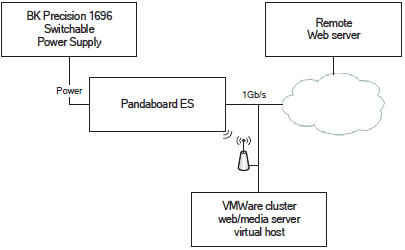
\includegraphics[scale=1,keepaspectratio]{proxy_setup}
\caption{Overview of the measurement setup}
\label{fig:proxy_setup}
\end{figure}

\addcontentsline{toc}{section}{Performance Evaluation For Web Requests}
\subsection*{Performance Evaluation For Web Request}
To perform a representative evaluation of frequent HTTP
web requests, web requests for Google’s home page were utilized.
The goal of this particular measurement scenario is to evaluate
the performance impact of frequent requests through the local
proxy server, which has to perform the additional connection
tasks each time a request is made. A direct
measurement application for Android was developed, which will request http://www.google.com without further resolving any
HTTP objects within. Individual requests are followed by a
sleep period of 2 seconds for both, direct requests and requests
through the mobile SOCKSv5 proxy service. As requests are
made without utilizing a browser, no caching is involved
client-side.

\addcontentsline{toc}{subsection}{Fixed Network}
\subsection*{Fixed Network}
In the fixed network scenario, the Pandaboard is connected
through wired Ethernet to the campus network while performing
the web requests. The requests typically coincide
with high power consumption levels, as illustrated in Figure \ref{fig:proxy_energy_cons_socks}
for an exemplary 100 web requests with both configurations.
We observe that both approaches exhibit an initial “spike”
behavior and an otherwise low level (with some general noise
due to overall device activities). There is no immediately
visible trend for the momentary power consumptions, as in
both approaches, there are several bursty periods of slightly
elevated consumptions on top of the actual web requests.
Next, we evaluate the total (compounded) energy consumption
that is observed when performing these requests for a
certain period of time. We illustrate 100 subsequent requests
directly and through the mobile proxy server in Figure \ref{fig:proxy_comp_energy_cons}.
Initially, it is observed that despite the short-term fluctuations,
there is a linear increase in the energy consumed
while using either approach. More significantly, there is no
immediately noticeable significant difference between the
approaches, which is indicated by the almost indistinguishable
values in the plot. Lastly, comparing the overhead between
the approaches numerically in Table \ref{tab:requests_summary}, where the
300 highest levels of energy consumption measured for periods
of placing 300 requests were analyzed. It's also notable that the direct approach
results in a higher average level of energy consumption (albeit
with a larger variability), whereas the proxy-based approach
yields a lower average and variability of energy usage values
determined. Overall, this results in an overhead of o =
−0.0563, which presents an initially counter-intuitive result.
(Differently worded, by utilizing the mobile proxy server
consuming additional CPU cycles, potential energy savings
of 5.6\% could be realized without requiring any additional
modifications.) Taking into account that partially significant
variability exists due to some outliers in the total duration
(as some measurement points can exhibit significant delays or
coincide with other unrelated system activities), both approaches are very similar.

\begin{figure}
\centering
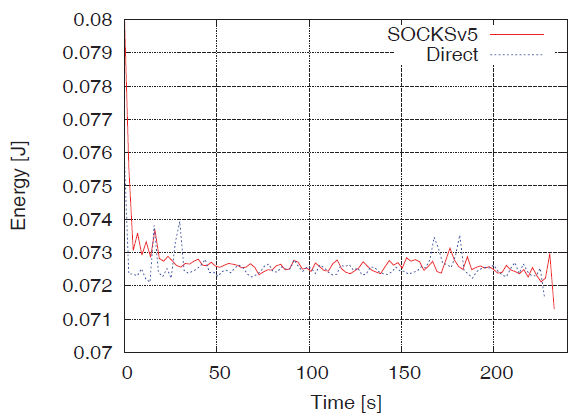
\includegraphics[scale=1,keepaspectratio,width=\columnwidth]{proxy_energy_cons_socks}
\caption{Energy consumption while performing 100 web requests directly or through a mobile SOCKSv5 service, smoothed over time.}
\label{fig:proxy_energy_cons_socks}
\end{figure}

\begin{figure}
\centering
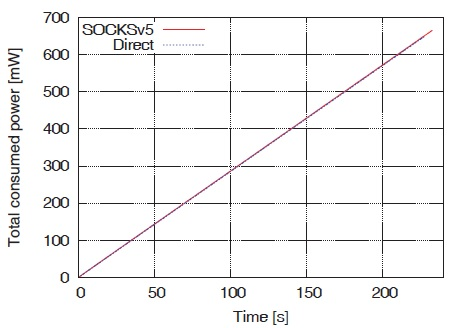
\includegraphics[scale=1,keepaspectratio,width=\columnwidth]{proxy_comp_energy_cons}
\caption{Compounded energy consumption for performing 100 web requests directly or through a mobile SOCKSv5 service.}
\label{fig:proxy_comp_energy_cons}
\end{figure}

\begin{table}[h]
\begin{tabular}{|c|c|c|c|c|}
\hline
 Interface & Approach  & Average[J]  & Standard Deviation [J] & Confidence Interval (99 \%)  \\ \hline
 LAN & Direct & 0.0912 & 0.0139 & 0.0021 \\ \hline
 LAN & Proxy & 0.0860 & 0.0062 & 0.0009 \\ \hline
 WLAN & Direct & 0.0900 & 0.0125 & 0.0019 \\ \hline
 WLAN & Proxy & 0.0902 & 0.0089 & 0.0013 \\ \hline
\end{tabular}
\caption{Summary values for 300 direct and proxy-routed web requests over traditional ethernet and wireless LAN networks.}
\label{tab:requests_summary}
\end{table}

\addcontentsline{toc}{subsection}{Wireless Network}
\subsection*{Wireless Network}
Shifting the evaluation to HTTP requests made over the
wireless network interface, we present our results in Table \ref{tab:requests_summary}.
(We note that a graphical evaluation would yield results similar
to those presented in Figures \ref{fig:proxy_energy_cons_socks} and \ref{fig:proxy_comp_energy_cons}.) We initially note that
both approaches are very close with respect to their measured
average energy consumption, resulting standard deviations,
and narrow confidence intervals. \newline
Comparing these results with those obtained for the Ethernet
scenario, which outlines the base case without active wireless
communications overheads, we do not note a significant difference
in the average energy usage for the individual web
requests.

\addcontentsline{toc}{section}{Impact of Web Request Variations}
\subsection*{Impact of Web Request Variations}
Motivated by the closeness of requests, the next step is to more
closely evaluate the impact of the web request size over a
wireless LAN on the overall power consumption. To limit
the impact that external networks can have (such as different
delays), the direct performance comparison is performed within
the on-campus VM environment illustrated in Figure \ref{fig:proxy_setup}. A
dedicated virtual machine uses the Apache2 web server and
hosts a Python script that generates a requested number of
bytes, additionally eliminating potential caching impacts. 100 repeated measurements are performed for each different web request size and significant outliers are deleted.

\addcontentsline{toc}{subsection}{Power Consumption}
\subsection*{Power Consumption}

\begin{figure}
\centering
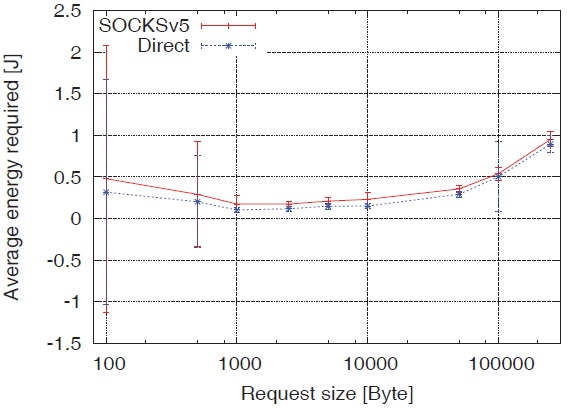
\includegraphics[scale=1,keepaspectratio,width=\columnwidth]{energy_cons_direct_vs_socks}
\caption{Average energy consumption and standard deviation for requesting different amounts of data from a local server using a direct or mobile SOCKSv5 proxy server.}
\label{fig:energy_cons_direct_vs_socks}
\end{figure}

\begin{figure}
\centering
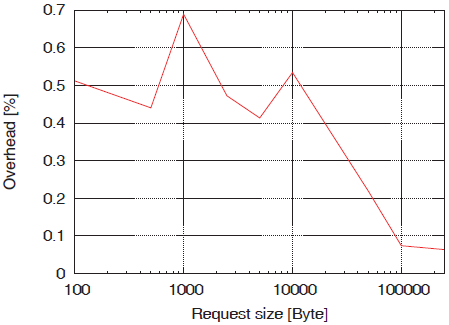
\includegraphics[scale=1,keepaspectratio,width=\columnwidth]{energy_cons_overhead}
\caption{Average energy consumption overhead for requesting different
amounts of data from a local server}
\label{fig:energy_cons_overhead}
\end{figure}

The average energy used per different request size is illustrated in in Figure \ref*{fig:energy_cons_direct_vs_socks}. It's observed that the mobile SOCKSv5 proxy approach always incurs a penalty
over the direct connection, which is readily explained by the
additional local processing overhead on the device. Furthermore,
it can be noted that both depicted connection methods follow
a “slump”-like behavior. Taking the overall variability of
measurements into account, until the amount of requested data
approaches the single packet payload region, the lowest energy
usage is recorded. This initial behavior can be explained
by the overhead to establish the initial server connection,
which is dominant for the small request size regions. With
a further increase of the payload to very large sizes, the
number of required transmissions drastically increases, which
now accounts for the majority of the energy consumption
(rather than the initial connection setup). This increase in the
number of packets is now causing longer periods of energy expensive
network activities, causing the rise in energy consumption
illustrated. The overall absolute difference between
the employment of a mobile proxy and direct connection,
however, remains fairly constant, which indicates that the
processing overhead for local packet processing prior delivery
to an application is rather negligible.
Next, the overhead incurred by the mobile
proxy server (as in Equation 1) in Figure \ref{fig:energy_cons_overhead}.Initially,
an overall “hump”-like behavior is observable which decreases as
the request sizes increase. Part of this behavior is explained
by the rather large variability (which isn't illustrated
here for clarity) in the regions of smaller request sizes. The overall diminishing overhead is explainable by the increase in the web request sizes with the actual overhead in the
processing and local loop-back data connections for the proxy
service. As the proxy service requires an initial connection
setup before performing the pass-through connection from the
remote server, additional time and processing resources are
required before the connection can be fully passed through
the proxy. Both resources incur processing and delay penalties
which in turn have negative power consumption impacts.
Larger request sizes result in increased numbers of packets
to transmit, which “smoothes” the fixed setup overhead over
more packets, which results in the decreasing overhead. At
250 kB of requested data, an observable reduction occurs to just below
six percent. Overall, that based on these measurements, it's observed that the implementation of a mobile proxy server directly on a
mobile device does not result in considerable additional power
demands for larger-sized web requests, which are common
today.

\addcontentsline{toc}{section}{Delay Difference}
\subsection*{Delay Difference}
With most interactive settings, the overhead in terms of
additional delays can have a negative impact on user utility
or perceived quality of service. In networked mobile settings,
increased delays additionally have a negative battery impact
through the direct correlation between the two.
The average delay differences between the proxy and the direct
connections for different request sizes is illustrated in Figure \ref{fig:time_difference_requests}. Initially,
there is a fairly steady level of added average delays to the
mobile proxy service in the region of 25 ms with higher levels of standard deviation occurring where the larger amounts
of data requested; an overall maximum of about 37 ms can
be noted for requesting 250 kB of data. The variability for
the delays is a combination of the script producing the larger
chunks of data with now slightly increased variability, as well
as the increased number of packets sent for each approach
incurring an additional network delay variation.
Overall, it can be concluded that the observed low level of additional
delay represents the fairly constant overhead of setting
up the proxy service on the mobile device and processing the
initial connection requests.

\begin{figure}
\centering
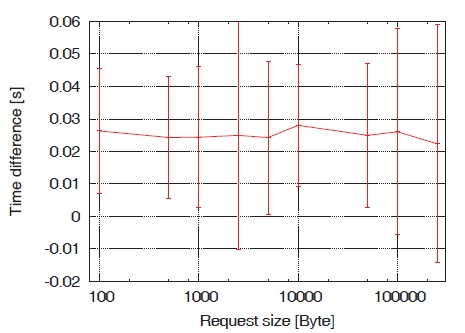
\includegraphics[scale=1,keepaspectratio, width=\columnwidth]{time_difference_requests}
\caption{Average time difference and standard deviation between the direct and the proxy approach for requesting different amounts of data from a local server.}
\label{fig:time_difference_requests}
\end{figure}

\addcontentsline{toc}{section}{Media Streaming}
\subsection*{Media Streaming}
The next step is to evaluate the impact of a long duration
connection through the mobile SOCKSv5 server, in contrast
to the previous evaluation of frequent connection requests.
Here, a continuous data stream needs to be forwarded to a
local application, with the initial setup overhead becoming
negligible. The playback of the web video on the Pandaboard
is performed using the Firefox for Android web browser. For
measurements of the incurred proxy overhead, the browser
is reconfigured to utilize the local SOCKSv5 proxy service,
similar to the previous web request scenarios. The HTML5
video is in turn displayed on the browser for the entire
duration.

\begin{figure}
\centering
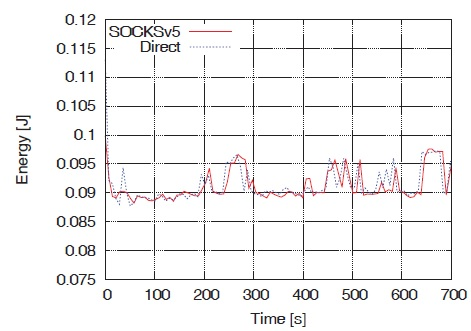
\includegraphics[scale=1,keepaspectratio,width=\columnwidth]{video_streaming_cons_socks}
\caption{Energy consumption while performing the video streaming of the
Tears of Steel open-source video sequence directly and through a mobile
SOCKSv5 proxy server, smoothed over time.}
\label{fig:video_streaming_cons_socks}
\end{figure}

\addcontentsline{toc}{section}{Fixed Network}
\subsection*{Fixed Network}
The sampled power consumption for video
streaming over a wired Ethernet network is illustrated in Figure \ref{fig:video_streaming_cons_socks}. Observing the graph, we can
see that most of the measured power consumption values
fall into a range between 3.25 W and 3.75 W for both
approaches. Both approaches additionally exhibit overall periods
of heightened power consumption, e.g., from about
250s to about 290s. This time frame coincides with a fast
camera movement following an actor (very high level of
background content change, motion) and represents a more
challenging video decoding task, in turn leading to higher
power consumption. Comparatively, however, it's also observable that no
significant differences exist between the two approaches. The aggregated
energy consumption resulting from media streaming
results in a linear behavior, which additionally is almost
indistinguishable between the two approaches as observed
for the prior web requests scenario. As indicated by the
comparable energy consumption over time in Figure \ref{fig:video_streaming_cons_socks}, the
additional video decoding power requirements let the overall
power consumption differences remain minor. We in turn omit
a visual representation that closely resembles Figure \ref{fig:proxy_comp_energy_cons} due
to space constraints. The aggregated performance
values for this scenario in Table \ref{tab:agg_perf_results}. NEED TO CHANGE THIS TO TABLE FORMAT IN LATEX INSTEAD OF PICTURE) Looking at the table, I note that the average
energy used is very similar for either approach, with slightly
elevated values for the direct approach. Taking the standard
deviation and the very narrow 99\% confidence intervals into
account, we note that the proxy-based streaming incurs no
significant penalties. Comparing this streaming example to the
individual web requests, I note that overall, the proxy-based
approach now is at the same overall level that I observed
for the direct case.

\begin{figure}
\centering
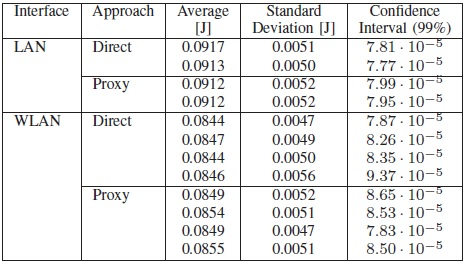
\includegraphics[scale=1,keepaspectratio]{agg_perf_results}
\caption{Summary values for HTML5 video streaming of the open-source Tears of Steel movie (video-only) over an ethernet and a wireless network.}
\label{tab:agg_perf_results}
\end{figure}

\addcontentsline{toc}{section}{Wireless Network}
\subsection*{Wireless Network}
As in the previous web request scenario, I additionally
investigate the alternative approach whereby the video streaming
is now utilizing a local wireless network.  The
measurement results in Table \ref{tab:agg_perf_results} for equal numbers of measurement
points. (Also note that for means of better comparison,
the number of measurement points are limited to be equal.) I
note that the overall averages are fairly close and furthermore
characterized by relatively narrow confidence intervals. The
resulting overhead, when comparing the averages of the direct
and proxy-based video streaming is 0.0081, or less than one
percent. Comparing the overall WLAN levels to the wired
measurements, I note a decrease in the overall power consumption.
This behavior is explained with the full availability of
all network interfaces, whereby the employed operating system
seems unable to properly put all different interfaces into a nopower
state.
Overall, I conclude that the introduction of the mobile
proxy server has only limited negative impacts on the power
consumption of about one percent when streaming multimedia
due to the significantly higher impact of the decoding processes
on the energy consumption and the negligible packet
processing overheads.



\addcontentsline{toc}{section}{Conclusions and Future Work}
\subsection*{Conclusions and Future Work}
I approximated the energy consumption overhead of
mobile optimization frameworks through a mobile SOCKSv5
proxy server as a low-end baseline. The selected implementation
is based on JAVA and performs all network traffic
forwarding on the application layer within the Dalvik VM for
Android devices. I found that the overall usage of a proxy
service on the mobile device in a web request scenario does
not incur any significant power consumption penalties. For
HTML5 video streaming (continuous packet processing), I
note an overhead of about one percent. I determined that any
existing overhead is relatively constant and explained through
the initial communication setup overheads, rather than ondevice
processing overheads, which were found to be approximately one
percent. A basic optimization framework would in turn only
need to overcome this very low overhead to enable energy
savings potentials.In future research avenues, I plan to investigate further energy savings potentials based on mobile device proxying,
in combination with caching and application layer content
awareness in tandem with a remote server.